\documentclass[12pt,a4paper]{standalone}
\usepackage[latin1]{inputenc}
\usepackage{amsmath}
\usepackage{amsfonts}
\usepackage{amssymb}
\usepackage{graphicx}
\author{José Antonio García Hernández}
\usepackage{tikz}
\begin{document}

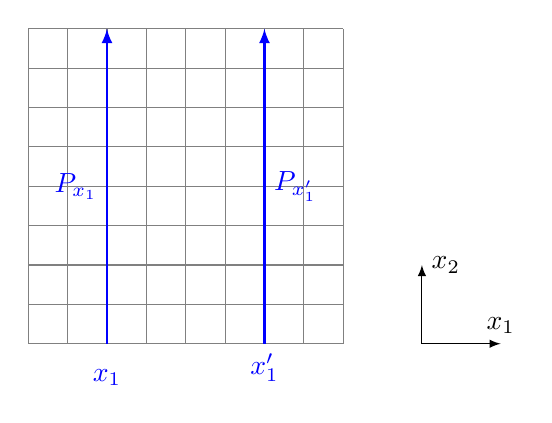
\begin{tikzpicture}
    \draw[step=0.5cm,color=gray] (0,0) grid (4,4);
    %\draw[step=1cm,color=gray,dashed] (-1,-1) grid (5,5);
    \draw[-latex,thick,blue] (1,0) --(1,4);
    \draw[-latex,thick,blue] (3,0) node[below] {$x'_1$} --(3,4);

    \draw[blue] (1,-0.43) node[] {$x_1$};

    \draw[blue] (1,2) node[left] {$P_{x_1}$};    
    \draw[blue] (3,2) node[right] {$P_{x'_1}$};
    \draw[-latex] (5,0)--(6,0) node[above]{$x_1$};
    \draw[-latex] (5,0)--(5,1) node[right]{$x_2$};
\end{tikzpicture}
\end{document}
